\chapter{Batch: Simulated CT Solution}

\textit{Further experiments with batch filtration was performed using simulated CT reservior water. The content of the simulated CT water was based on the primary species present in water from a CT reservoir being \ce{Ca^{2+}},  \ce{Na+}, \ce{Cl-}, \ce{SO4^{2-}} and \ce{SiO2}.
The aim of these filtrations was to investigate how pH influence the rejection of the respective ions. 
\textcolor{blue}{Noget med ICR her måske den dele op i 2}
}


\section{Experimental Method}
%\prettyinpink{Noget med water recovery}




The concentration of the specific ions in the simulated CT water was based on samples of authentic CT reservoir water measured in relation to internal work within Grundfos, and is summarized in \cref{tab:multisalt_composition}. 
This experiment will investigate the rejection of ions with changing environment, 10 L simulated CT water was filtered in a batch process similar to filtration of the binary ions.
The effect of pH on the membrane rejection was investigated, with pH at three different levels: pH 9.2, pH 10, and pH 10.5. 
The pH values investigated are chosen to be in a range that would likely impact the charge of silica species and thereby their rejection as mentioned in \cref{Silica_teori_ladning}. 
This best guess approach is not ideal from an experimental design point of view, but allows one to quickly gain information on how the system responds to the change in pH.
In order to regulate, ensure stable pH and mimic the buffering capacity of authentic CT reservoir water, a carbonate-bicarboante buffer solution was used when producing the simulated CT water. 
This was deemed necessary due to results of batch filtrations with binary ion solutions, see \cref{Kapitel_batch_single_salt}.
%CT water has a buffer capacity which is not replicated when the simulated CT water exclusively consists of salts added to RO-water.
A 0.008 M carbonate-bicarboante buffer was used as the base for all simulated CT water and adjusted to the desired pH before filtration. 
%This strength of 0.008 M was based on bicarbonate concentration in authentic CT water. 



%This was chosen to examine how membrane performance (i.e. rejection of ions) changes as filtration progresses and ion concentrations increase in the feed stream.

% The goal was to see the impact on Cl and silica rejection which should be able to be investigated.
% The Cl rejection is expected to be dependent on the concentration of other species present in the feed tank / at the membrane wall \textcolor{blue}{ref til teori/ explanation} and therefor will likely change as the filtration progresses.
% Silica rejection however, is expected to be less dependant on the matrix effects, but instead on the solution pH as this is responsible for the degree to which silica is charged.



\begin{table}[H]
\centering
\caption{Ionic compositions of authentic CT water compared to selected composition in simulated CT water. The \ce{HCO3-} and \ce{Na+} concentration change based on desired pH.}
\label{tab:multisalt_composition}
\rowcolors{2}{gray!25}{white}
\begin{tabular}{r|cccc}
\rowcolor{gray!50}
\textbf{Ion Species}   & \textbf{Authentic CT water} & \textbf{ID: 1} & \textbf{ID: 2} &\textbf{ ID: 3} \\ \hline
\ce{Ca^{2+}} {[}mM{]}   & 0.35               & 0.40   & 0.40  & 0.40    \\
\ce{Na+} {[}mM{]}   & 10.81              & 11.77  & 14.76 & 16.63   \\
\ce{Cl-} {[}mM{]}   & 2.48               & 2.50   & 2.50  & 2.50    \\
\ce{SO_4^{2-}} {[}mM{]}  & 0.64               & 0.70   & 0.70  & 0.70    \\

\ce{SiO2} {[}mM{]} & 0.68               & 0.70   & 0.70  & 0.70    \\
\ce{HCO_3^-}{[}mM{]}  & 7.29               & 6.07   & 3.08  & 1.21   \\
pH & & 9.2&10 &10.5 \\
\ce{Cl-}/Anion ratio &&&& \\
\end{tabular}
\end{table}



\textbf{ICR (Increase Chloride Rejection)}

To further investigate the rejection of chloride additional filtrations with varying \ce{Cl^{-}/(SO4^{2-}+Cl-)} ratio was performed, by varying the \ce{SO4^{-2}} concentration see \cref{tab:ICR_phase_1_conc}. 
For \textcolor{blue}{1} filtration more frequent sampling was performed, every 20 min for the first 6 hours, this was done to investigate the development of the chloride rejection during the start of the filtration. 

\textcolor{blue}{noget med vores permeat forsøg...}

%A 10 L batch filtration with sampling every 20 min for 6 hours of both feed and permeate. Where  "the complex ion matrix" filtrations had sampling after 2.5 or 3 hours.
%The filtration carried out with the same procedure as for "the complex ion matrix" with the concentrations presented in \cref{tab:ICR_phase_1_conc} and at pH 9.5. 

\begin{table}[H]
\centering
\caption{Ionic Compositions of Matrices}
\label{tab:ICR_phase_1_conc}
\rowcolors{2}{gray!25}{white}
\begin{tabular}{l|cccc}
\rowcolor{gray!50}
\textbf{Ion Species}   & \textbf{ID: 4} &\textbf{ID: 5}  \\ \hline
\ce{Na+} {[}mM{]}  & 25          &      \\
\ce{Cl-} {[}mM{]} & 5              &     \\
\ce{SO_4^{2-}} {[}mM{]}  & 5        &         \\
\ce{Ca^{2+}} {[}mM{]} & 0.5         &          \\
\ce{SiO2} {[}mM{]} & 1.25           &        \\
\ce{HCO_3^-} {[}mM{]} & 5.9          &      \\
pH & 9.75 & 9.75\\
\ce{Cl-}/Anion ratio & & \\
\end{tabular}
\end{table}





\section{Data Processing }

\rod{skal vi gøre som bruno og oplyse 1 samlet rejection for hver ion?\\
Vi mangler usikkerheder på IC + Silica\\
Fejlkilder der er udeladt:\\
Water mystery.\\
HCl content used to adjust pH before experiment was not measured.
}
Apart from varying pH level between filtrations ID: 1-3, another slight difference is that the ID 2 filtration (pH 10) had smaller initial feed volume of 8.5 L leading to shorter filtration time compared to ID 1 and 2 with initial feed volume of 10 L.
%, and thereby would not have time to reach the same concentrations.
%The first samples are taken at a water recovery of 35 \% for low and middle pH and a 25\% for high pH.
%Samples were then collected somewhat evenly until filtration stopped.
Due to a large dead volume of the filtration system compared to initial feed volume, it was difficult to replicate a water recovery of 90 \% for all filtrations, the last samples where taken at 87\%, 76\% and  80\% for ID:1, 2 and 3 respectively. 

The initial pH of each experiment was slightly of the targeted pH and increased during each experiment (increase of $\sim$0.12 pH unit).
The pH increase is likely a result of the increasing concentration of silica as the filtration progresses.
% For the low pH filtration the increase was from 9.31 to pH 9.44.
% The middle pH experiment saw increase from 10.08 to 10.24 but the experiment duration was slightly shorter.
% In the high pH experiment the increase was from pH 10.47 to pH 10.59.

TMP increased during filtration for all experiments, likely a result of increased osmotic pressure of the feed solution.

\textcolor{blue}{vi tager kun måling i feed/retentate det er det samme.}

\subsection{Bicarbonate}

Samples for bicarbonate analysis was taken from the feed container in each filtration at various times, see \rod{Appendix: multi salt} for raw data.
It is generally observed for all filtrations (ID: 1-3) that the bicarbonate concentration increases as filtration progresses.
This large increase in measured bicarbonate may be a result of increasing silica concentrations, as silica concentration most likely impact the bicarboante/alkalinity analysis as seen for the binary ion experiment \cref{Kapitel_batch_single_salt}.
%The measured bicarbonate by alkalinity is likely not independent from the concentration of silica.
There seems to be a linear relationship between silica content and measured bicarbonate, see \rod{Appendix: multisalt}


\subsection{Silica}

The silica rejections increases in filtrations with higher pH, see \Cref{fig:silica_rejection_multi_salt}.
Furthermore in all three experiments silica rejection increases as filtration progresses likely due to slight increase in pH during filtration.
For ID: 1 with pH 9.2 the rejection is initially 21.2\% then decreases as the filtration progresses to 8.8\% at 60\% water recovery, before increasing to 27.4 \%. 
For the ID: 2 filtration with pH 10 silica rejection increases steadily from 47.5\% to 58.7\%
Silica rejection was greatest for ID: 3 which had highest pH at 10.5, with initial silica rejection at 64\% reaching 72.7\%. 
This is likely a result of an increased fraction of charged silica species present at higher pH values, as described in theory section, see \cref{fig:silica_pH_fraktion}. 
%which are more easily retained by the negative membrane surface(which may also be affected by solution pH).

\begin{figure}[H]
    \centering
    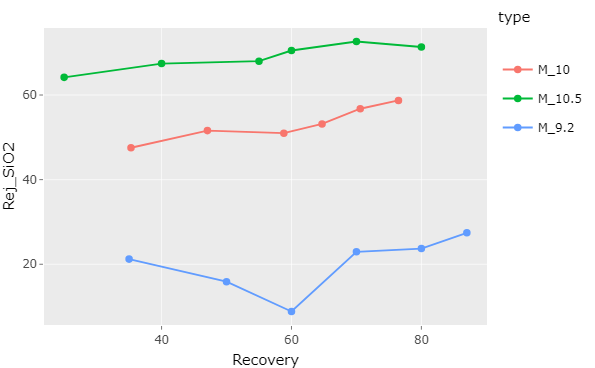
\includegraphics[width=0.8\textwidth]{Billeder/data/multi_salt/silica_rejection.png}
    \caption{Rejection of silica at different pH values}
    \label{fig:silica_rejection_multi_salt}
\end{figure}



\subsection{Ionic Rejection}

Samples were taken from feed tank and permeate stream and ion rejections are illustrated for filtrations ID: 1-3 at the tree pH levels, see \cref{fig:multi_salt_pH_ion_rejections_samlet_med_sulfat_og_silica}.

\textbf{Sulphate}
The sulphate concentrations of the permeate samples was below the Limit of determination (LOD) of 5 mg/L and this value will instead be used to estimate rejections.
Assuming permeate concentrations of 5 mg/L sulphate rejection goes from 95 \% - 98 \% during filtration at all pH values.


\begin{figure}[H]
    \centering
    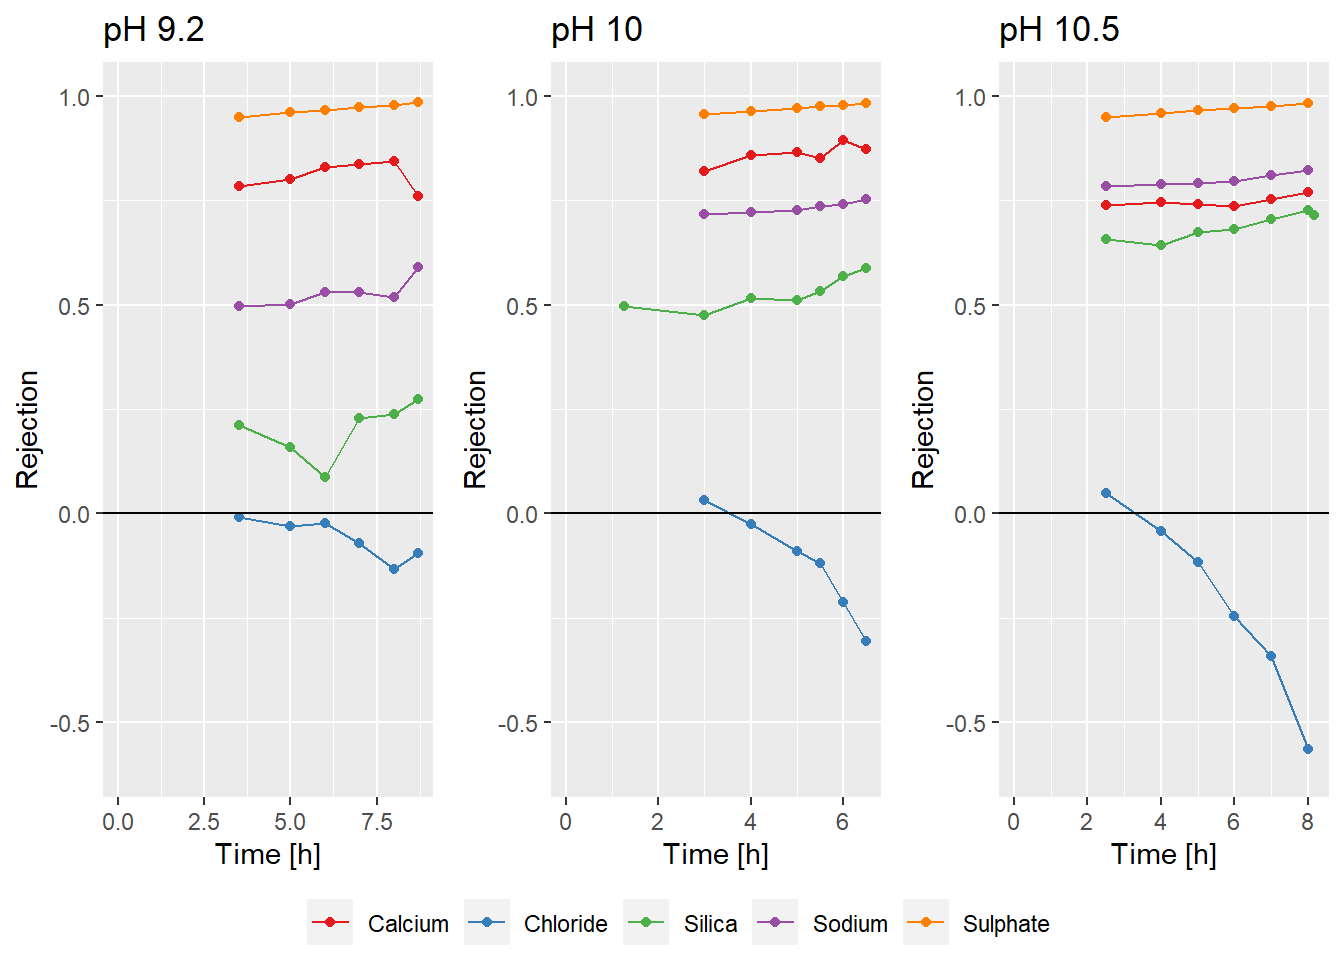
\includegraphics[width=0.8\textwidth]{Billeder/data/multi_salt/multisalt_ion_rejections_with_sulphate_and_silica.png}
    \caption{Ion Rejections for all complex ion filtrations, with sulphate rejection assuming [SO4] = 5 mg/L for permeate at all times.}
    \label{fig:multi_salt_pH_ion_rejections_samlet_med_sulfat_og_silica}
\end{figure}



\textbf{Chloride:}
Chloride rejection decreases as filtration progresses for filtrations at all pH levels.
For ID:1 pH 9.2 the Cl rejection is just below 0 at first measured sample and it reaches lowest values of -13\% at 80\% water recovery.
The ID:2 filtration with pH 10 has initial Cl rejection of 3\%  which decreases to -30\% at a the final water recovery of 76\%.
For ID:3 at pH 10.5 the first measured rejection was 5\% and this decreased to -56\%.
% pH 9.2: -0.007 ->-0.096
% pH 10: 0.03 ->-0.3
% pH 10.5: 0.05 ->-0.56
When comparing the first measured Cl rejection between filtrations ID:1-3 there is a trend with increase in Cl rejection at higher pH value. 
Contrary it is evident that chloride rejection decreases dramatically at higher pH level. 
The presence of other anions present is assumed to be the major cause for poor rejection of Chloride.
Assuming that sulphate rejection is somewhat unaffected by pH change, the major reason for decreased Cl rejection with pH increase is that a larger fraction of silica is present on an ionic form.
For all pH values rejection of the other ions (i.e. not Cl- or SiO2) increases slightly as each filtration progresses.

\textbf{Sodium:}
Sodium rejection increases with higher pH
At high pH there is greater Na rejection than Ca rejection unlike at the other two pH levels.

At filtration with the low pH level Na rejection starts at 49.7\% and increases to 59\%.
For the middle pH the first rejection value is 71.2\% and the increase is less substantial reaching 75.2\%
At the highest pH value there is a high initial Na rejection of 78.5\% rising slightly to 82.3\%.

% Feed concentrations:
% 344->626
% 361 -> 808
% 404 -> 1145


\textbf{Sulphate:}
The sulphate rejection is as previously mentioned based on constant permeate concentration of 5 mg/L.
Under this assumption the rejection is 95-98\% during each filtration and is unaffected by pH changes.

% Feed Sulphate concentrations:
% low pH: 98 -> 311
% middle pH: 71-> 274
% High pH: 69 -> 291
% based on concentration profile pH 10.5 has the largest increase in sulphate concentration during the filtration, but pH 9.2 reaches highest final concentration. 


\textbf{Calcium: }
For unknown reasons feed Ca concentrations are much greater in the low pH experiment than the other two experiments.
Initial concentrations are 24 mg/L in the low pH experiment but only 3.4 mg/L in the other two.

Rejection is similar between low and middle pH but is lower in the high pH experiment where it is lower than sodium rejection
For the low pH experiment rejection starts at 78\% and ends up at a value of 84, ignoring the last sample.
the middle pH calcium rejection is 82\% at water recovery of 35\% progressing to 88\%.
In the high pH experiment Ca rejection is 74\% to 77\% and thus is lower than the other two experiments for the entire duration.
The likely cause of the Ca rejection pH dependence is that an increasing flux of negative ions through the membrane result in a larger Donnan effect causing increased transportation of positive ions over the membrane.
The preferential transport of Ca over Na ions can be explained by the charge difference.
As Ca is divalent and has a similar radius to Na \rod{havde du fundet deres radius?} Ca has a greater charge density and would be affect by electrical potential to a greater extent.

\subsection{ICR}
For the additional experiment conducted everything is bad.

pH of the feed solution was 9.75 during the filtration.

Silica rejection was constant at 34\% rejection throughout the filtration.
As expected silica rejection was between the low and middle pH levels of the three CT experiments, further agreeing that silica rejection is primarily controlled by solution pH.
Sodium and calcium rejection was also between the performance of the low and middle pH filtrations.

The primary focus for the experiment was the  performance of the first part of the filtration, especially chloride rejection.
There is however no clear trend that can be seen from the chloride rejection in the first part of filtration.
Rejection increases and decreases multiple times and only shows predictable behaviour after a water recovery of 40\%, which is when sampling frequency was lowered.
The low quality of the samples may therefore be caused by the sampling frequency during the first part of filtration.
The limited water flux through the membrane may mean that the system needs longer between sampling to produce useful results.

\begin{figure}[H]
    \centering
    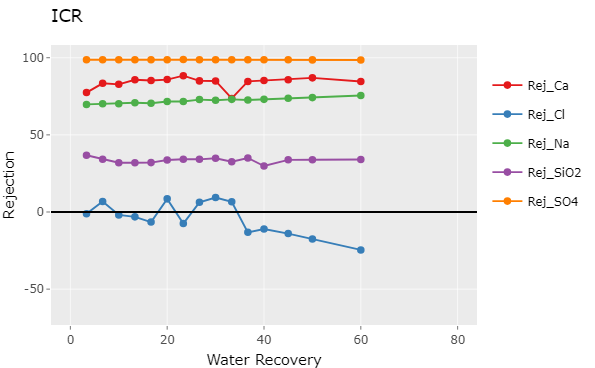
\includegraphics[width=0.7\textwidth]{Billeder/data/multi_salt/ICR_1_rejection.png}
    \caption{rejection of ions for the ICR experiment}
    \label{fig:my_ICR_rejection}
\end{figure}












% Feed Ca concentrations:
% pH 9.2: 24 -> 46 -> 30
% pH 10: 3.2 -> 19
% pH 10.5: 3.6 -> 7.8




% \begin{figure}[H]
%     \centering
%     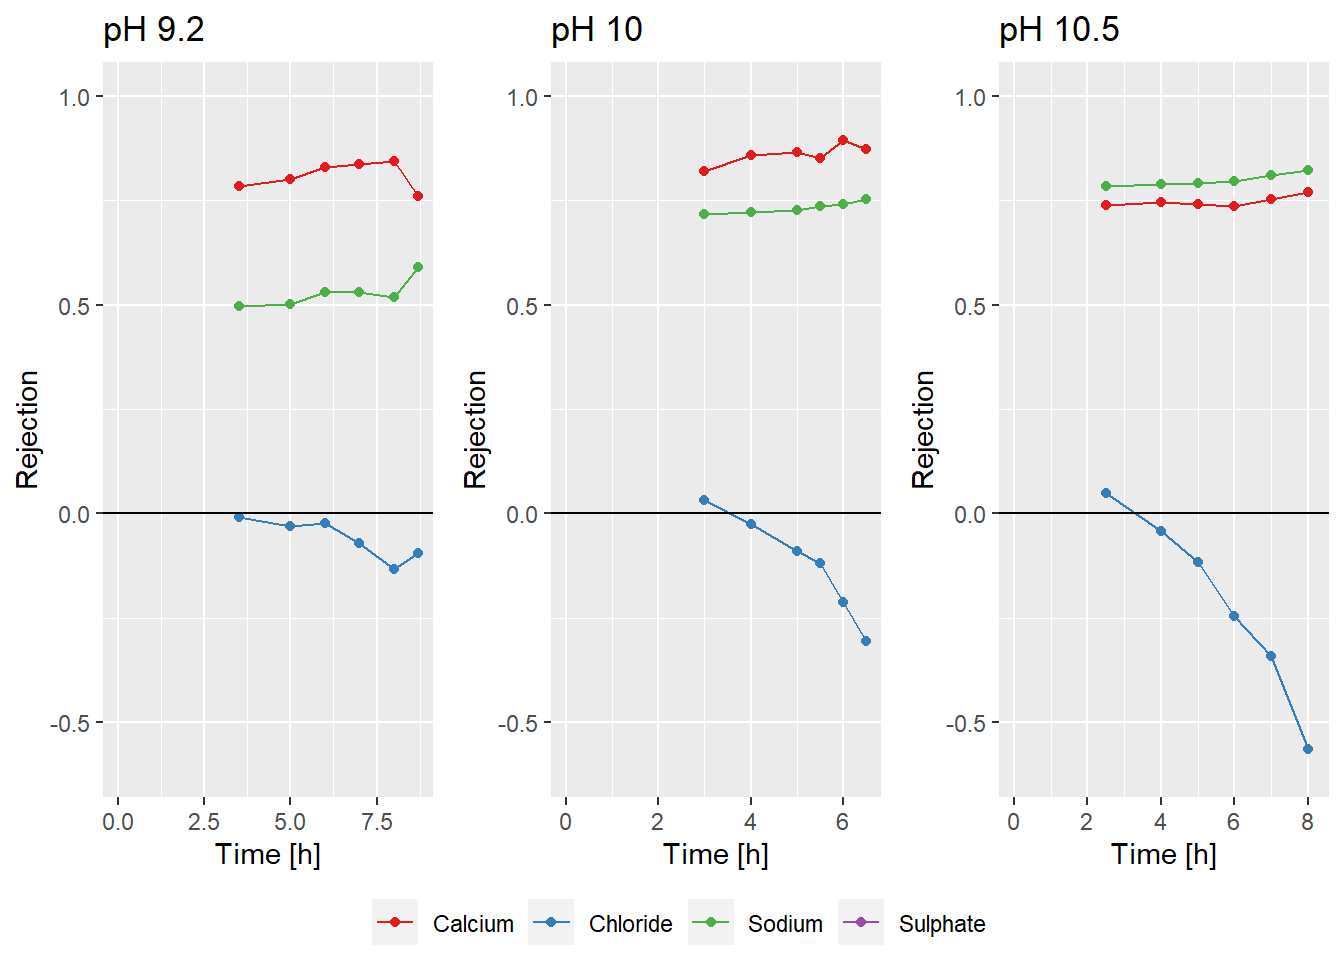
\includegraphics[width=0.8\textwidth]{Billeder/data/multi_salt/multisalt_ion_rejections.png}
%     \caption{Ion Rejections for all multisalt experiments}
%     \label{fig:multi_salt_pH_ion_rejections_samlet}
% \end{figure}

% \begin{figure}[H]
%     \centering
%     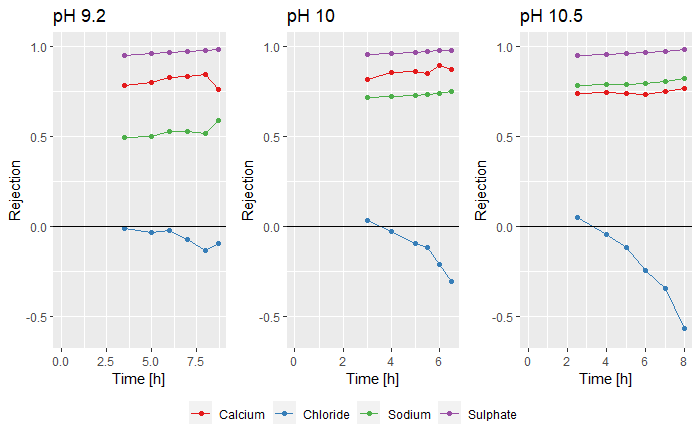
\includegraphics[width=0.8\textwidth]{Billeder/data/multi_salt/multisalt_ion_rejections_with_sulphate.png}
%     \caption{Ion Rejections for all multisalt experiments, now with sulphate rejection assuming [SO4] = 5 for permeate at all times}
%     \label{fig:multi_salt_pH_ion_rejections_samlet_med_sulfat}
% \end{figure}


